% % % % % % % % % % % % % % % % % % % % % % % % % % % % % % % % % % % % % % % % 
% LaTeX4EI Template for Cheat Sheets                                Version 1.0
%					
% Authors: Emanuel Regnath, Martin Zellner
% Contact: info@latex4ei.de
% Encode: UTF-8, tabwidth = 4, newline = LF	
% % % % % % % % % % % % % % % % % % % % % % % % % % % % % % % % % % % % % % % % 


% ======================================================================
% Document Settings
% ======================================================================

% possible options: color/nocolor, english/german, threecolumn
% defaults: color, english
\documentclass[german]{latex4ei/latex4ei_sheet}
\usepackage{stix}
\usepackage[ngerman]{babel} 
% set document information
\title{ELMA \\ Cheat Sheet}
\author{Raoul Duke}
\myemail{0x4723@gmail.com}
\mywebsite{www.github.com/doppelplus/CheatSheets}

% ======================================================================
% Define MathOperator
% ======================================================================

\DeclareMathOperator{\arcsec}{arcsec}
\DeclareMathOperator{\arccot}{arccot}
\DeclareMathOperator{\arccsc}{arccsc}
\DeclareMathOperator{\arcsinh}{asinh}
\DeclareMathOperator{\arccoth}{acoth}
\DeclareMathOperator{\arctanh}{atanh}
\DeclareMathOperator{\arccosh}{acosh}

% ======================================================================
% Begin
% ======================================================================
\begin{document}


% Title
% ----------------------------------------------------------------------
\maketitle   % requires ./img/Logo.pdf

% Tipps und Tricks
% ----------------------------------------------------------------------
\section{Allgemeines}
	\begin{sectionbox}
		\subsection{Drehstrom}\label{Drehstrom}
			\begin{bluebox}{Elektrische Eingangsleistung von Drehfeldmaschinen}
				\item $\cos \varphi$: Leistungsfaktor (Winkel zwischen $U_N$ und  $I_N$)
				\item $P_{el} = 3 \cdot U_S \cdot I_S \cdot \cos \varphi  =  \sqrt{3}  \cdot U_N \cdot I_N \cdot \cos \varphi$
				\item Bei Sternschaltung: $U_S = \frac{1}{\sqrt{3}}U_N \quad I_S = I_N$
				\item Bei Dreiecksschaltung:  $U_S = I_N \quad I_S = \frac{1}{\sqrt{3}}I_N$
			\end{bluebox}


			\begin{symbolbox}{Leistung im Drehstromsystem}
				\item $S= \sqrt{3} \cdot U_N \cdot I_N = \sqrt{P^2 +Q^2}$
				\item $P = 3 \cdot U_S \cdot I_S \cdot \cos \varphi = \sqrt{3} \cdot U_N \cdot I_N \cdot \cos \varphi$
				\item $Q = \sqrt{3}\cdot U_N\cdot I_N \cdot \sin \varphi = 3\cdot U_S\cdot I_S\cdot \sin \varphi$
			\end{symbolbox}

			\begin{bluebox}{Effektivwerte}
				\item Wechselstrom, der an einem Widerstand die gleichen Stromwärmeverluste verursacht wie ein genauso großer Gleichstrom:
				\item $I^2_{eff}\cdot R = I^2_{DC}\cdot R$
				\item Zeitabhängiger Strom:
				\item $i = I(t) =  \hat{I} \cdot \cos(\omega t) = \sqrt{2}\cdot I_{eff}\cdot \cos(\omega t)$
				\item Spitzen \& Effektivwert: $\hat{I} = \sqrt{2}\cdot I_{eff}\quad \hat{U} = \sqrt{2}\cdot U_{eff}$
			\end{bluebox}
			\begin{symbolbox}{Ströme in den Phasen}
				\item $i_{L1}= \hat{I}\cos(\omega t)$
				\item $i_{L2}= \hat{I}\cos(\omega t-\frac{2}{3}\pi)$
				\item $i_{L3}= \hat{I}\cos(\omega t+\frac{2}{3}\pi)$
			\end{symbolbox}

		\subsection{Synchronmaschinen}
			\begin{bluebox}
				\item $f_1$:\quad Frequenz des Ständerstroms
				\item $p$: \quad Polpaarzahl(Anzahl Rotorpolpaare)
				\item $n_1$:\quad Drehzahl des Stratorfeldes $n_1 = \frac{f_1}{p}$
				\item $d$:\quad Luftspaltdurchmesser
				\item $\tau_p$: \quad Polteilung$\tau_p =\frac{\pi \cdot d}{2p}$
				\item Geschwindigkeit der Rotoroberfläche: $v=2\tau_p \cdot f_1$
			\end{bluebox}

		\subsection{Asynchronmaschinen}
			\begin{symbolbox}
				\item $I_0 =\frac{U_1}{\sqrt{R_s^2+S_x^2}}$:\quad Leerlaufstrom
				\item $s$:\quad Schlupf $s = \frac{n_1-n}{n_1}$
				\item $n$:\quad Rotor- bzw. Wellendrehzahl $n = (1-s)\cdot \frac{f_1}{p}$
				\item Anfahrt im Kippmoment: $f = f_n (1-s_k)$
			\end{symbolbox}
	\end{sectionbox}


	\begin{sectionbox}
		\section{Elektrisches Antriebssystem}
		\subsection{Betriebsbereiche elektrischer Antriebssysteme}
			\begin{tablebox}{ll}
				S1-Dauerbetrieb:& $M\leq M_N$, $x\leq n_N$\\
				Überlastbereich:& $M>M_N$, $n\leq n_N$\\
				Feldschwächung Überlasbereich:& $M>M_N$, $n>n_N$\\
				Feldschwächung Dauerbetrieb:& $M\leq M_N$, $n>n_N$\\
			\end{tablebox}

	\end{sectionbox}
	\begin{sectionbox}
		\subsection{Verluste, Leistung, Wirkungsgrad und Drehmomnent}
			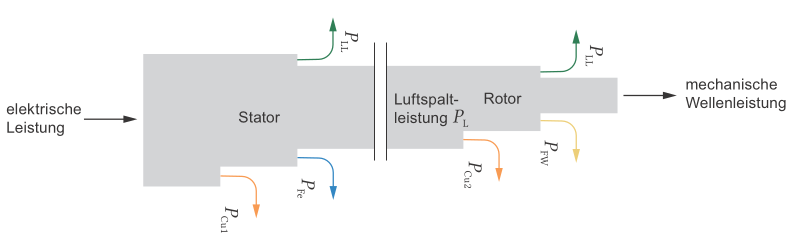
\includegraphics[width=190px]{ELM_Verluste.png}
			\begin{symbolbox}
				\item Generatorbetrieb: $P_{el} = P_{mech} -P_{Vel}-P_{Vmech}$
				\item Motorbetrieb: $P_{mech} = P_{el} -P_{Vel} -P_{Vmech}$
			\end{symbolbox}
			\begin{bluebox}{Wirkungsgrad}
				\item $\eta = \frac{P_{ab}}{P_{zu}}$
				\item $\eta_{Motorbetrieb} = \frac{P_{mech}}{P_{el}} = \frac{P_{el} -P_{Vel} -P_{Vmech}}{P_{el}}$
				\item$\eta_{Generatorbetrieb} = \frac{P_{el}}{P_{mech}} = \frac{P_{el}}{P_{el}+P_{Vel}+P_{Vmech}}$
			\end{bluebox}
			
			\begin{symbolbox}{Mechanische Wellenleistung}
				\item $M$ = mechanisches Wellendrehmoment (aussen)
				\item $\varphi$ = Mechanischer Verdrehwinkel
				\item $\omega$ = mechanische Winkelgeschwindigkeit ($\omega = \frac{\varphi}{t}$)
				\item $n$ = Drehzahl der Welle, $[n] = 1/s$
				\item $P_{mech} = M \cdot \omega = M \cdot 2\cdot \pi\cdot n$
			\end{symbolbox}

			\begin{bluebox}{Dynamischer Prozess}
					\item $P_{el}$ = aus dem Netz aufgenommene elektrische Leistung
					\item $P_{Load} $ = von der Arbeitsmaschine (Load) genutzte Leistung
					\item $P_{VTransmission} $ = mech. Verluste der Übertragungselemente
					\item $P_{Vel} $ = elektrisch bedingte Motorverluste
					\item $P_{Vmech} $ = mechanisch bedingte Motorverluste
					\item $P_{VCDM} $ = Verluste im Frequenzumrichter
					\item $W_{kinL} $ = kin. Energie der Arbeitsmaschine
					\item $W_{kinTransmission} $ = kin. Energie der Übertragungselemente
					\item $W_{kinMotor} $ = kinetische Energie des Elektromotors
					\item $W_{potL} $ = potenzielle Energie der Arbeitsmaschine (z. B. Aufzug)
					\item $W_{elMotor} $ = in den Spulen gespeicherte elektromagnetische Energie des Motors
					\item $P_{el} = P_{Load} + P_{VTransmission} + P_{Vel} + P_{Vmech} + P_{VCDM} + \frac{d}{dt}\cdot (W_{kinL}+W_{kinTransmission} + W_{kinMotor} + W_{potL} + W_{elMotor})$
			\end{bluebox}
			
			\begin{symbolbox}{Kinetische Energie \& Trägheitsmoment}
				\item $J$: Massenträgheitsmoment drehender Körper $[J] = 1kg\cdot m^2$
				\item $\omega$: Mechanische Winkelgeschwindigkeit ($\omega = 2\pi \cdot n$)
				\item $v$: Geschwindigkeit in $\frac{m}{s}$
				\item $m$: Masse in $kg$
				\item $g$: Erdbeschleunigung ($9,81\frac{m}{s^2}$)
				\item Rotierendes System: \quad $W_{kin} = \frac{1}{2}J\omega^2$
				\item Lieare Bewegung: \quad $W_{kin} = \frac{1}{2} \cdot m \cdot v$
				\item Potentielle Energie: \quad $m\cdot g\cdot h$
				\item Im Motor gespeicherte el. Energie: \quad $W_{el} = \frac{1}{2}LI^2$
				\item Im Kondensator gespeicherte el. Energie: \quad $W_{el} = \frac{1}{2}CU^2$
			\end{symbolbox}
			\begin{cookbox}{Frequenzumrichter}
				\item Schlupf zum gewünschten Drehmoment ausrechnen, da der Schlupf vom Drehmoment abhängig ist.
				\item Statordrehzahl berechnen: $n_1 = n\cdot(1+s)$
				\item Drehfeldfrequenz berechnen: $f_1 = n_1 \cdot p$
				\item ...Profit
			\end{cookbox}
	\end{sectionbox}

\section{Getriebe}
	\begin{sectionbox}

		\begin{bluebox}
		$P_2 \cong P_1$
		$i$: Übersetzung
		$J$: Schwungmasse
		\end{bluebox}
		\hspace{1.5cm} 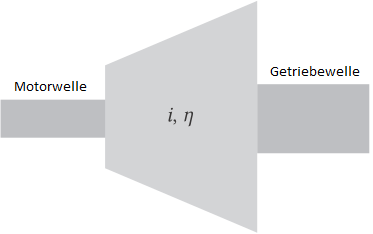
\includegraphics[width=75px]{Getriebe.png} 
			\begin{tablebox}{ll}
				$n_1$, $M_1$, $J_1$&$n_2= n_1/i$\\
				$P_1 = 2\pi n_1\cdot M_1$&$M_2=\eta\cdot M_1 \cdot i$\\
				&$J_2=J_1\cdot i^2$\\
				&$P_2=P_1\cdot \eta= 2\pi n_2\cdot M_2$\\
			\end{tablebox}
	\end{sectionbox}

	\section{Physikalische Grundlagen}
	\begin{sectionbox}
		\subsection{Kraft, Leistung, Energie}
			$F= m \cdot a$

			$[F] = 1N,[m]= 1\,kg$, $[a]= 1\,m/s^2$

			$F= m \cdot \mu \cdot g$ ($\mu$ = Reibkoeffizient)

			\begin{symbolbox}{Drehmoment bei Rotationsbewegung}
				\item $M$: Drehmoment
				\item $r$: Hebelarm
				\item $[M] = 1\,N \cdot m$, $[F]= 1\,N$, $[r]=1\,m$
				\item $P = F\cdot v = M\cdot \omega$, ($\omega = 2\pi\cdot n$)
				\item $[P]= 1\,W$. $[v]= 1\,m/s$, $[\omega]=1/s$, $[n]=1/s$ 
				\item $W= P\cdot t$
				\item $[W]= 1\,W\cdot s = 1J(Joule)$, $[t] = 1\,s$
				\item $1\,kwh = 3\,600\,000 J$
			\end{symbolbox}
			\begin{bluebox}{Maxwell Gleichungen}
				\item Größen:
				\item D: el. Verschiebungsdichte (el. Flussdichte); $[D] = A \cdot s/m^2$
				\item E: el. Feldstärke; $[E ] = 1\,V/m$
				\item B: mag. Flussdichte; $[B] = 1\,V\cdot s/m2 = 1\,T$ (Tesla)
				\item H: mag. Feldstärke; $[H] = 1\,A/m$
				\item M: Magnetisierung eines Permanentmagneten; $[M] = 1\,A/m$
				\item F: Fläche
				\item $\phi$: mag. Fluss
				\item $J_P$: mag. Polarisation; $[J_P] = 1\,V \cdot s/m2 = 1\,T (Tesla)$
				\item $\mu_0$: mag. Feldkonstante
				\item $μ_0 =  4\pi \cdot 10^{-7}(V\cdot s)/(A\cdot m)\simeq 1,257\cdot 10^{-6}(V\cdot s)/(A\cdot m)$
				\item Energiedichte im Magnetfeld: $\rho_m = \frac{B^2}{2\mu_0\mu_r}$
				\item Differentielle Form
				\item $div \vec{D} = \vec{\nabla} \cdot \vec{D} = \rho$
				\item $div \vec{B} = \vec{\nabla} \cdot \vec{B} = 0$
				\item $rot \vec{E} = \vec{\nabla} \times \vec{E} = \frac{\partial \vec{D}}{\partial t}$
				\item $rot \vec{H} = \vec{\nabla} \times \vec{H} = \vec{J} + \frac{\partial \vec{D}}{\partial t}$
				\item Integrale Form
				\item $\oiintup\limits_{\partial v}\vec{D} \cdot d \vec{f} = \iiint\limits_v p \,dv$
				\item $\oiintup\limits_{\partial v}\vec{B} \cdot d \vec{f} = 0$
				\item $\oint\limits_{\partial f} \vec{E}\cdot d \vec{s} = - \iint\limits_f \frac{\partial \vec{B}}{\partial t}\cdot d \vec{f}$
				\item $\oint\limits_{\partial f} \vec{H}\cdot d \vec{s} = \iint\limits_{f}\vec{J}\cdot d \vec{f}+ \iint\limits_{f}\frac{\partial \vec{D}}{\partial}\cdot d \vec{f}$
				\item Materialgleichungen:
				\item $\vec{D}= \varepsilon_0 \varepsilon_r\vec{E}$
				\item $\vec{B}= \mu_0\vec{H}+\vec{J}_P=\mu_0(\vec{H}+\vec{M})= \mu_0\mu_r\vec{H}$
			\end{bluebox}
	\end{sectionbox}
	\begin{sectionbox}
		\subsection{Durchflutungssatz}
			\begin{symbolbox}
				\item $\sum\limits_i H_i \cdot I_i = w \cdot I =\Theta$
				\item $B = \frac{\phi}{F}$
			\end{symbolbox}
	\end{sectionbox}

	\begin{sectionbox}
		\subsection{Magnetische Werkstoffe}
			\subsubsection{Weichmagneten}
				\textbf{Technische Eigenschaften von Elektroblech}
				\begin{tablebox}{ll}
					Dichte & $7,87\,g/cm^2$\\
					El. Leitfähigkeit & $10 \cdot 10^6 \cdot 1/(\Omega m)$\\
					Wärmeleitfähigkeit & $80\,W(m\cdot K)$\\
					Schmelzpunkt & $1538^\circ C$\\
					max. Flussichte bis zur Sättigung & 1,25 \dots 2,2 T\\
					Preis/kg & 1,5 EUR
				\end{tablebox}
				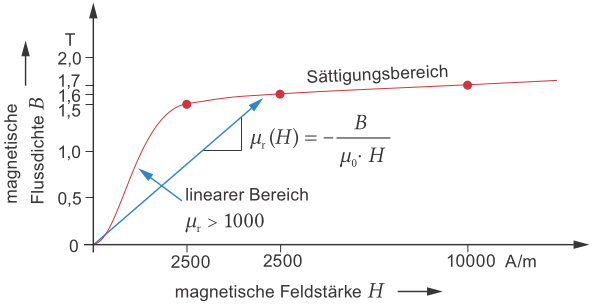
\includegraphics[width=175px]{ElektroblechDiag.png}
				\begin{bluebox}{Ummagnetisierungsverluste}
					10\% bis 20\% Anteil am Gesamtverlust
				\end{bluebox}

				\begin{symbolbox}{Hystereseverluste}
					\item 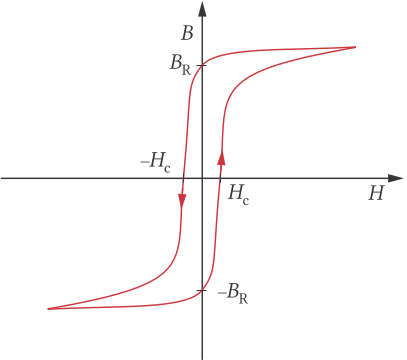
\includegraphics[width=100px]{HystereseBlech.png}
					\item \begin{quote}
						Von den Herstellern der Bleche wird ein Materialkennwert $\sigma_hyst$ angegeben, 
						der die spezifischen Hystereseverluste pro kg Elektroblech bei 1,5 T maximaler Flussdichte und
						50 Hz Frequenz angibt.
					\end{quote}
					\item $P_{hyst} = \sigma_{hyst}\cdot m (\frac{f}{50Hz}\cdot \frac{B_{max}}{1,5\,T})$
				\end{symbolbox}

				\begin{bluebox}{Wirbelstromverluste}
					\item \begin{quote}
						Ähnlich wie bei den Hystereseverlusten gibt der Stahlhersteller einen Materialkennwert
						$\sigma_{wb}$ für die spezifischen Wirbelstromverluste an. 
						Die gesamten Wirbelstromverluste errechnen sich entsprechend aus:
					\item $P_{wb} = \sigma_{wb}\cdot m\cdot (\frac{f}{50Hz})^2\cdot (\frac{B_{max}}{1,5\,T})$
					\end{quote}
				\end{bluebox}
			\end{sectionbox}
			\begin{sectionbox}
				\subsubsection{Hartmagneten}
				\begin{tablebox}{p{2.8cm}|p{1cm}|p{1cm}|p{1cm}}
					Formelzeichen & &$SmCo_{5/17}$& $NdFeB$\\
					Koerzitivfeldstärke (kA/m) & 100-350 & 600-850 & 500-1100\\
					Remanenzflussdichte (T) & 0,2-0,4 & 0,9-1,2 & 0,7-1,5\\
					Energiedichte ($kJ/m^3$)& 10-40 &140-300& 300-450\\				
				\end{tablebox}
			\end{sectionbox}
			\begin{sectionbox}
				\subsection{Induktionsgesetz}

					\begin{symbolbox}
						\item 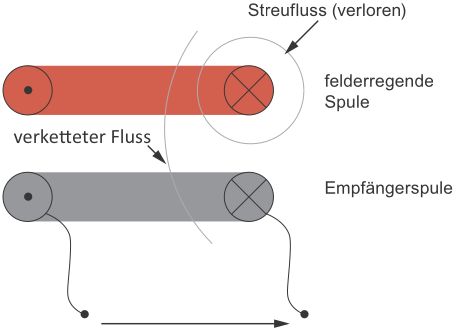
\includegraphics[width=100px]{Induktionsgesetz} 
						\item \hspace{1cm}$u_i= -\frac{d\psi}{dt}$
						\item $w$: Windungszahl
						\item $\psi$: Flussverkettung / verketteter Fluss
						\item $u_i$: induzierte Spannung
						\item $\oint\limits_{C} \vec{E}\cdot d \vec{l} = \frac{d\phi}{dt}$ 
						\item $\psi = w\cdot \phi$
						\item $u_i = -\frac{d\psi}{dt} = -w\cdot \frac{d\phi}{dt}$
						\item $\psi_{max}$ wenn Spulen genau gegenüber liegen.
						\item $u_i = -\frac{d}{dt}\psi(x,i)= -\frac{\partial\psi}{\partial i}\cdot \frac{di}{dt}-\frac{\partial \psi}{\partial x}\cdot \frac{dx}{dt}$
						\item $\frac{\partial \psi}{\partial i} = const. \rightarrow L = \frac{\psi}{i}$
						\item Rechteckige Geometrie: $\frac{\partial \psi}{\partial x} = \frac{B\cdot A}{x} = B \cdot l$
						\item Induktionsgesetz: $u_i = -L\cdot \frac{di}{dt}-B\cdot l\cdot v$ 
						\item Induktionsgesetz für einen Leiter: $u = B\cdot l\cdot v$
					\end{symbolbox}
				\subsection{Lorenzkraft}
					\begin{bluebox}
						\item $i$: Strom im Leiter
						\item $B$: magnetische Flussdichte
						\item $l$: die im Magnetfeld befindliche Länge des Leiters
						\item $M$: Drehmoment
						\item $d$: Rotordurchmesser
						\item $z$: Anzahl der Leiter
						\item $P$: Leistung
						\item $n$: Umdrehungen pro Sekunde
						\item $\vec{F} = i\cdot (\vec{l}\times \vec{B})$
						\item $M \cong  \frac{d}{2}\cdot sum F \cong \frac{d}{2}\cdot z\cdot I\cdot l \cdot B$
						\item $P = M \cdot \omega = M \cdot 2\pi n$
					\end{bluebox}
				\subsection{Reluktanzkraft}
					\begin{symbolbox}
						\item $S$: Fläche, durch die die Feldlinien austreten
						\item $B$: mag. Flussdichte
						\item $\mu_0$: mag. Feldkonstante $\simeq 1,257\cdot 10^{-6}(V\cdot s)/(A\cdot m)$
						\item $\vec{F} = -\frac{1}{2}\int\limits_V \vec{H}^2 \cdot grad \mu dV$
						\item In der Praxis (Übergang Elektroblech($\mu_r \rightarrow\infty$) zu Luft($\mu =  1))$: $F = \frac{B^2\cdot S}{2\mu_0}$
					\end{symbolbox}
				\end{sectionbox}

				\begin{sectionbox}
					\subsection{Leistungsdichte}
						\begin{bluebox}
							\item $f_S$: Flächenkraft
							\item $B$: Mittlere mag. Flussidchte (0,8-1,1 T) (Begrenzt durch Leistungsfaktor ($\cos \varphi$) \& Eisensättigung)
							\item $A$: Strombelag ($\sum i/(\pi d)$), Kühlungsabhängig (50-100 kA/m Dauerbetrieb, 100-200 kA/m Spitzenbelastung)
							\item $f_S = B\cdot A$
							\item $f_{Smax} \approx 200\, kN/m^2$
							\item $C$: Ausnutzungsfaktor (Esson Zahl)
							\item $M$: Drehmoment
							\item $\xi$: Wickelfaktor ca. 0,96
							\item $d$: Rotordurchmesser
							\item $l$: die im Magnetfeld befindliche Länge des Leiters
							\item $C = \pi^2 \cdot \xi\cdot A \cdot B$
							\item $M = \frac{1}{2\pi}\cdot C\cdot d^2\cdot l \cdot \eta \cdot \cos \varphi$
							\item $P = n \cdot C \cdot d^2 \cdot l \cdot \eta \cdot \cos \varphi$
							\item $\rho = n \cdot C \cdot \eta\cdot \cos \varphi$
						\end{bluebox}
				\end{sectionbox}

\section{Drehfeldwicklungen}
	\begin{sectionbox}
		
			\subsection{Lochzahl}
				\begin{symbolbox}
					\item $q$: Lochzahl
					\item $N$: Anzahl der Nuten
					\item $2p$: Anzahl der mag. Pole
					\item $m$: Phasenzahl (i. D. R. 3)
					\item  $q = \frac{N}{2 p m}$
				\end{symbolbox}
			\subsection{Wickelfaktor}
				\begin{bluebox}
					\item $v$: Rotorgeschwindigkeit, $p$ = Polpaarzahl
					\item $l$: Länge der Spule, $N$ = Anzahl der Statornuten
					\item $u = B\cdot l \cdot v$ Spannung, die in einem Leiter im Feld der drehenden Rotormagnete induziert wird.
					\item $v = 2\tau_p\cdot f_1$
					\item $W$: Spulenweite ($W = \frac{N}{p}$)
					\item $\xi$: Wickelfaktor
					\item 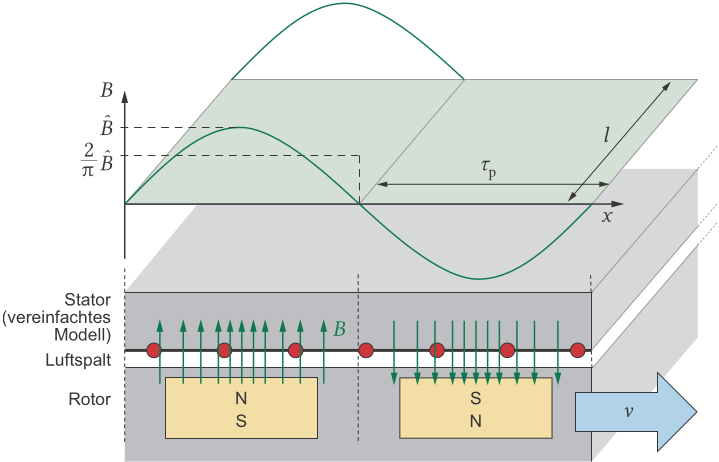
\includegraphics[width=125px]{WickelfaktorModell.png}
					\item $\hat{U} = \hat{B}\cdot l\cdot 2\tau_p \cdot f$
					\item $\phi_{Pol} = \frac{2}{\pi} \cdot \hat{B}\cdot l \cdot \tau_p$
					\item $U_{Leiter} = \frac{\pi}{\sqrt{2}}\cdot f_1 \cdot \phi_{Pol}$
					\item $\phi_{Pol} = \frac{\sqrt{2}}{\pi}\cdot \frac{U_{Leiter}}{f_1}$
					\item $\xi_{Gruppe} = \frac{sin\left(\frac{q\cdot \frac{\alpha}{2}}{2}\right)}{q\cdot \sin\left(\frac{\alpha}{2}\right)}$, $\alpha = 2\pi \cdot \frac{p}{N}$
					\item $\xi_{Schraegung} = \frac{\sin(\frac{\varepsilon}{2})}{\frac{\varepsilon}{2}}$, $\varepsilon = \frac{\tau_{Schraegung}}{\tau_p}\cdot \pi$
					\item $\xi_{Sehnung} = \sin\left(\frac{W}{\tau_p}\cdot \frac{\pi}{2}\right)$
					\item $\xi = \xi_{Gruppe} \cdot \xi_{Schraegung} \cdot \xi_{Sehnung}$
					\item $E_h = 2w\cdot U_{Leiter}\cdot \xi$, $E_h$ = Spannungsinduktion des Hauptfeldes
				\end{bluebox}
	\end{sectionbox}

	\section{Asynchronmaschinen}
		\begin{sectionbox}
			\subsection{Parameterbestimmung}
				\begin{symbolbox}{Hauptinduktivität}
					\item $m$: Phasenzahl
					\item $\delta'$: Um Carter Faktor erweiterter Luftspalt
					\item $\tau_p$: Polteilung
					\item $l_{Fe}$: Aktive Länge (Eisenlänge)
					\item $2p$: Polzahl
					\item $\xi$: Wickelfaktor
					\item $w$: Windungszahl eines Strangs
					\item $N_1$: Anzahl der Statornuten
					\item $z_N$: Leiterzahl pro Nut
					\item $a$: Anzahl pro Phase geschalteter Zweige
					\item $p$: Polpaarzahl
					\item $q$: Lochzahl
					\item $L_h = \frac{m}{2}\cdot \frac{\mu_0}{\delta'}\cdot \frac{2}{\pi}\cdot \tau_p \cdot l_{Fe}\cdot \frac{4(w\xi)^2}{2p}$
					\item $w= \frac{N_1\cdot z_N}{2a\cdot m} = p\cdot q \cdot \frac{z_N}{a}$
				\end{symbolbox}
				\begin{bluebox}{Statorwiderstand, Rotorwiderstand \& Wicklungstemperatur}
					\item $R_1$ = Statorwiderstand
					\item $l$: Drahtlänge
					\item $A$: Drahtfläche $A = d^2\cdot \frac{\pi}{4}$
					\item $d$: Drahtdicke ohne Isolation
					\item $\theta_1$: Raumtemperatur
					\item $\gamma$, $\kappa$: Elektrische Leitfähigkeit des Leitermaterials
					\item $\gamma{Cu20} = 56\cdot 10^6\cdot 1/(\Omega m)$, $\kappa_{Al20} = 33\cdot 10^6\cdot 1/(\Omega m)$
					\item $\alpha$: Temperaturbeiwert $\alpha_Cu = 3,93\cdot 10^{-3}K^{-1}$
					\item $R_1 = \frac{1}{\gamma}\cdot \frac{l}{A}$
					\item $\rho = \frac{1}{\gamma}\rightarrow \rho(\vartheta) = \rho_{20}\lfloor 1+\alpha(\vartheta -20^\circ C) \rfloor $
					\item Mit. Wicklungstemp.:  $\vartheta_2 = (\vartheta_1+k)\cdot \frac{R_2}{R_1}-k$ ($k_{Cu} = 235K$, $k_{Al} = 225K$)
					\item $N_r$: Nutenzahl des Käfigs
					\item $R_R$: Widerstand des Bogens im Kurzschlussring zw. zwei Stäben
					\item $R_S$: Einzelner Stabwiderstand
					\item Rotorwiderstand: $R_r = 2R_R+4\left(sin\left(\rho\frac{\pi}{N_r}\right)\right)^2\cdot R_S$  
					\item Nutstreuwert: $\lambda_{sN}$; typ. 0,5-5
					\item Streuinduktivität Strator: $L_{s\sigma} = L_{sN}+L_{sS}+L_{sD}$
					\item StatorNutstreuung: $L_{sN} =2\mu_0\cdot l_{Fe}\cdot \frac{w^2}{p\cdot q}\cdot \lambda_{sN}$n
					\item $l_{wk}$: Länge des Wickelkopfes
					\item $\lambda_{sS}$: Stirnstreuleitwert des Stators
					\begin{itemize}
						\item 0,35 bei 4-poligen Zweischichtwicklungen
						\item 0,28 bei 2-poligen Zweischichtwicklungen mit Runddraht
						\item 0,23 bei 2-poligen Zweischichtwicklungen mit Formspulen
						\item ansonsten etwa 0,3
					\end{itemize}
					\item Stirnstreuung: $L_{sS} = 2\mu_0\cdot l_{wk}\cdot \frac{w^2}{p}\cdot \lambda_{sS}$
					\item Stator-Oberwellenstreuung: $\sigma_{sO}=$ abh. von q zw. 0,005 - 0,05 
					\item Streuinduktivität Rotor: $L_{r\sigma} = L_{rN}+L_{rD}$
					\item $d$: Statorinnenduchmesser
					\item Rotornutstreuung: $L_{rN} = 4\mu_0 l_{Fe}\cdot \left(\sin\left(p\frac{\pi}{N_r}\right)\right)^2\cdot \sigma_{rO}$
					\item $\sigma_{rO} = \left( \frac{p\frac{\pi}{N_r}}{\sin(p\frac{\pi}{N_r})}\right)^2-1$
				\end{bluebox}
				\subsection{Leistung und Drehmoment}
						\item Stator $I^2R$ Verluste: $P_{sI2R} = 3\cdot I_s^2\cdot R_s$
						\item Mag. Übertragene Leistung auf Rotor: $P_D = P_S-P_{sI2R}-P_Fe-P_{LL}$
						\item $P_D = 3\cdot I_r'^2\cdot \frac{R_r'}{s}$
						\item $P_i = (1-s)\cdot P_D = 3\cdot I_r'^2\cdot R_r'\cdot \frac{1-s}{s}$
						\item $M = \frac{1}{\omega}\cdot (1-s)\cdot P_D$
						\item $P = (1-s)\cdot P_D-P_{fw} = M\cdot \omega$ ($P_{fw}$ = Friction \& Windage)
	\end{sectionbox}

	\begin{sectionbox}
		\subsection{Stationäres Betriebsverhalten}
			\begin{symbolbox}{Kippmoment \& Kippschlupf}
				\item Generatorbetrieb: -\qquad Motorbetrieb: +
				\item Kippmoment (Näherung): $M_i(s) = \pm M_k\cdot \frac{2}{\frac{s}{s_k}+\frac{s_k}{s}}$
				\item Kippschlupf: $s_k \cong \pm \frac{R'_r}{\omega_S\cdot L_{s\sigma}+L'_{r\sigma}}$
			\end{symbolbox}
			\begin{bluebox}{Dimensionierung der Antriebsstrangkomponenten}
				\item $M_{eff} = \sqrt{\frac{1}{T}\sum\limits_{i=1}^m M_i^2\cdot \Delta t_i}$
				\item $n_{mittel} = |\overline{n}_{L,i}|= \frac{1}{T}\sum\limits_{i=1}^m|n_{L,i}|\cdot \Delta t_i$
				\item $P_{eff} = M_{eff}\cdot 2\pi n_{mittel}$
			\end{bluebox}
			\textbf{Verhalten der wichtigsten Motorkenngrößen im Grunddrehzahl- und Feldschwächbereich}
			\begin{tablebox}{p{2cm}|l|l}
				&\textbf{Grunddrehzahlbereich} & \textbf{Feldschwächbereich}\\
				\hline
				Statorfrequenz $f_1$ & $0<f_1<f_n$ & $f_1 > f_n$\\
				Benötigte Statorspannung $U_1^{a)}$ & $(f_1/f_n)\cdot U_n$ & $U_1 = U_n$\\
				Kippmoment $M_k$ & $M_{kn}$ & $(f_n/f_1)^2\cdot M_{kn}$\\
				therm. zul. $I_{dauer\,th}$ & $I_n^{b)}$\\
				therm. zul. $M_{dauer\,th}$ & $M_n$ & $(f_n/f_1)\cdot M_n$\\
				therm. zul. $P_{dauer\,th}$ & $(f_1/f_n)\cdot P_n$ & $P_n^{b)}$
			\end{tablebox}
			a) Dabei beachte man den Boost-Faktor bei kleinen Frequenzen.
			b) Bei hohen Frequenzen müssen der thermisch zulässige Strom und damit auch die Leistung wegen zunehmender Eisen- und Reibungsverluste abgesenkt werden.
	\end{sectionbox}
	\begin{sectionbox}
		\subsection{Dynamisches Betriebsverhalten}
			\begin{symbolbox}{Bewegungsgleichung bei starrer Kopplung}
				\item $M_i$: inneres (elektromagnetisches) Drehmoment des Motors
				\item $M_{fw}$: Drehmoment zur Überwindung von Reibung und Lüftung
				\item $M_L$: Drehmomentbedarf der Last
				\item $J$: Trägheitsmoment
				\item 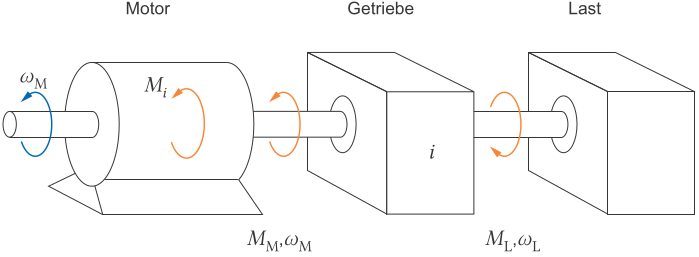
\includegraphics[width=150px]{DrehmomentDrehzalenLast.png}
				\item $M'_L = \frac{1}{i}\cdot M_L$
				\item $\omega_L' = i\cdot \omega_L = \omega_M$
				\item $J'_L=\frac{1}{i^2}\cdot J_L$
				\item $M_i-M_{fw}-\frac{1}{i}\cdot M_L= \left(J_M+\frac{1}{i^2}J_L\right)\frac{d\omega_M}{dt}$ Ohne Getriebe ist $i=1$
				\item Beschleunigungsmomemnt: $M_B = M_i-M_{fw}-\frac{1}{i}\cdot M_L$
				\item Hochlaufzeit: $t_H = \int\limits_{t1}^{t2}\,dt = J_{res,M}\cdot \int\limits_{\omega_1}^{\omega_2}\frac{1}{M_B(\omega_M)}\, d\omega_M$
				\item $t_H = \frac{J_{res,M}}{\overline{M}_B}\cdot \omega_N$ (Bei von 0 auf Bemessungsdrehzahl)
				\item $J_{Zyl} = \frac{1}{2}\cdot m r^2$\qquad $J_{Ring} = \frac{1}{2} m (r_a^2+r_i^2)$
				\item $J'_L = \frac{1}{i^2}\cdot J_L$
				\item $J_{ers, M} = \frac{m\cdot v^2}{\omega_M/i^2} = m\cdot \frac{r^2}{i^2} =\frac{1}{4}m\cdot \frac{d^2}{i^2}$
				\item Das \textbf{J}  der Last wird quadratisch mit der Untersetzung i auf die
				Motorwelle heruntergerechnet, Das \textbf{M}  der Last wird linear mit der Untersetzung i auf die Motorwelle
				heruntergerechnet. Die \textbf{N} der Last wird linear mit der Untersetzung i heraufgerechnet.
			\end{symbolbox}
	\end{sectionbox}
	\begin{sectionbox}
		\subsection{Aufteilung des Beschleunigungsmoments}
			\begin{symbolbox}
				\item Factor of Inertia: $FI = \frac{J_M+J_L/i^2}{J_M}$ 
				\item Bei ungekuppelter Motor $(J_L > 0\rightarrow FI = 1)$
				\item Bei $J_M = J_L\rightarrow FI = 2$
				\item $\frac{M_L}{M_M} =\frac{FI-1}{FI}$
			\end{symbolbox}
		\subsection{Schaltbetrieb mit Kupplungen}
		\begin{bluebox}
			\item $\gamma$ = elastischer Verdrehwinkel
			\item \begin{quote}
				Besonders kritisch sind Lose bei Schaltvorgängen. Aufgrund des anfänglichen Fehlens
			von Gegendrehmoment kann der Rotor sehr schnell beschleunigen. Er dreht praktisch
			leer los. Bereits nach wenigen Millisekunden und Winkelgraden ist bereits eine erhebliche 
			Rotationsenergie im Läufer vorhanden. Wenn die Lose aufgebraucht sind, wird der
			Motor schlagartig gebremst. Dabei wird die Rotationsenergie in Verformungsarbeit umgesetzt
			\end{quote}
			\item $W = \frac{1}{2}J\cdot \omega^2 = \frac{1}{2}M_{max}\cdot \gamma$
		\end{bluebox}
		\subsection{Ersatzschaltbild}
			\begin{symbolbox}
				\item 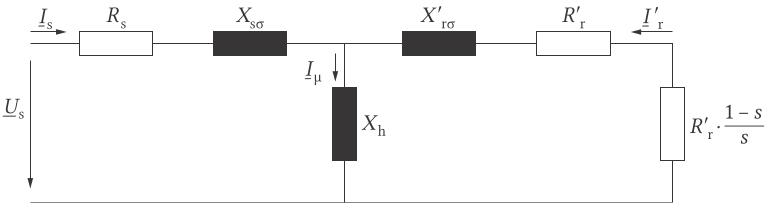
\includegraphics[width=180px]{AsynchronErsatzschaltbild.png}
				\item $\cos \varphi = \frac{R_r'}{\sqrt{R_r'^2+X_{r\sigma}^2}}$
				\item Rotorwiderstand: $\frac{R_r'}{s} = R_r' + R_r'\cdot \frac{1-s}{s}$
				\item Verantwortlich für Wärmeverluste $R_r'$
				\item Verantwortlich für $P_{mech}$: $R_r'\cdot \frac{1-s}{s}$
			\end{symbolbox}
	\end{sectionbox}

	\section{Transformatoren}
		\begin{sectionbox}
			\subsection{Allgemeines}
				\begin{bluebox}
					\item $\frac{U_1}{U_2} = \frac{N_1}{N_2} = \ddot{u} $
					\item $\frac{I_1}{I_2} = \frac{N_2}{N_1} = \frac{1}{\ddot{u} }$
					\item $\delta = \frac{N\cdot I}{H_L}$
					\item $H_L = \frac{B}{\mu_0}$
					\item $B = \frac{\phi}{A}$
				\end{bluebox}

			\subsection{Leerlaufmessung}
				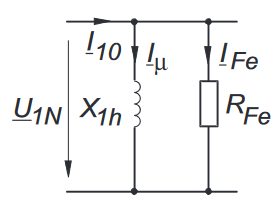
\includegraphics[height=50px]{TrafoLeerlaufErsatzschaltbild.png}
				\begin{symbolbox}
					\item Leerlaufstrom: $I_{10}$
					\item Verluste im Lerrlaufbetrieb: $P_0 = U_{1N}\cdot I_{10} \cdot \cos(\phi_0)$
					\item Eisenverlustwiderstand: $R_{Fe} = \frac{U_{1N}^2}{P_0} = \frac{U_{1N}}{I_{1N}\cdot \cos(\phi)}$
					\item Hauptreaktanz: $X_h = \frac{U_{1N}}{I_{1N}\cdot \sin(\phi)}$
					\item Hauptinduktivität: $L_h = \frac{X_h}{2\cdot \pi \cdot f}$
				\end{symbolbox}
		\end{sectionbox}

	\section{Synchronmaschinen}	
		\begin{sectionbox}
			\begin{symbolbox}{Allgemeines}
				\item $P_{mech} = 3 \cdot U_p \cdot I_N \cdot \cos \phi$
			\end{symbolbox}
			\begin{bluebox}{Kurzschlussverhältnis KC}
				\item Bemessungsspannung: $U_{1N}$
				\item Bemessungsstrom: $I_{1N}$
				\item Synchrone Reaktanz: $X_d$
				\item Kurzschlussstrom: $I_{K0} = \frac{U_{1N}}{X_d}$
				\item $K_C = \frac{I_{K0}}{I_{1N}} = \frac{U_{1N}}{X_d\cdot I_{1N}}$
			\end{bluebox}
		\end{sectionbox}
	\begin{sectionbox}
	\subsection{Besondere Eigenschaften von PMSM}
	\begin{symbolbox}
		\subsubsection{Wickelfaktor}
		\item Lochzahl: $q = \frac{N}{2\cdot p\cdot m} = \frac{z}{n}$
		\item Gruppenfaktor: $\xi_{Gruppe} = \frac{\sin\lfloor \frac{\pi}{2}-\frac{p\cdot \pi}{N} \cdot z \rfloor}{z\cdot \sin \left( \frac{\pi}{2}-\frac{p\cdot \pi}{N}\right)}$
		\item Sehnungsfaktor: $\xi_{Sehnung} = \sin\left(\frac{p\cdot \pi}{N}\right)$
		\item Wickelfaktor: $\xi =  \xi_{Gruppe} \cdot \xi_{Sehnung}$
	\end{symbolbox}
	
	\subsubsection{Bauformabhängiges Drehmoment}
		\begin{tablebox}{lll}
			FESM & $L_d > L_q$ & $M=\frac{3}{2}p\left(L_{FD}\cdot I_2I_q+(I_d\cdot I_q)\right)$\\
			PMSM o. Reluk. & $L_d = L_q$ & $M=\frac{3}{2}p\cdot \psi_{PM\cdot I_q}$\\
			PMSM m. Reluk. & $L_d < L_q$ & $M= \frac{3}{2}p\left(\psi_{PM}\cdot I_q+(L_d-L_q)\cdot I_d I_q\right)$\\
			synRM & $L_d<L_q$ & $M= \frac{3}{2}p(L_d-L_q)I_d\cdot I_q$
		\end{tablebox}
	\end{sectionbox}
	\begin{sectionbox}
		\subsection{Polradspannung $U_p$ und Polradwinkel $\vartheta_N$}
			\begin{cookbox}{Konstruktion des Zeigerdiagramms \& Berechnung}
				\item Nur die relative Lage zueinander ist wichtig.
				\item Reale Strangspannung auftragen
				\item Motorbetrieb: $+\varphi$ \quad Generatorbetrieb: $-\varphi$  
				\item Strangstrom mit $\varphi$ von Strangspannung auftragen
				\item $U_p = U_S + \underline{j} \underline{X_d}\cdot \underline{I_S}$
				\item $X_d \cdot I_S$ sitzt auf $U_S$ und ist orthogonal zu $I_S$ wg. $\underline{j}$
				\item Winkel zw. $X_d \cdot I_N$ und $U_S$ beträgt $90^\circ + \varphi$
				\item $U_p$ zw. Nullpunkt und Ende $X_d \cdot I_S$ auftragen.
				\item $U_p =\sqrt{U_S^2+(X_d\cdot I_S)^2-2U_S\cdot X_d \cdot I_S \cdot \cos(90^\circ+\varphi_N)}$
				\item $\vartheta_N = \arcsin\left(\frac{X_d\cdot I_N}{U_p}\cdot \sin(90^\circ + \varphi_N)\right)$
				\item $\underline{U_p} = U_p \cdot e^{j\vartheta}$
			\end{cookbox}
			$\frac{U_p}{U_1} = \frac{I_E}{I_{E0}}$
	\end{sectionbox}
		\vspace{5cm} % ToDo: Remove if needed
	\section{Gleichstrommaschinen}
		\begin{sectionbox}
			\subsection{Aufbau des Ständers}
				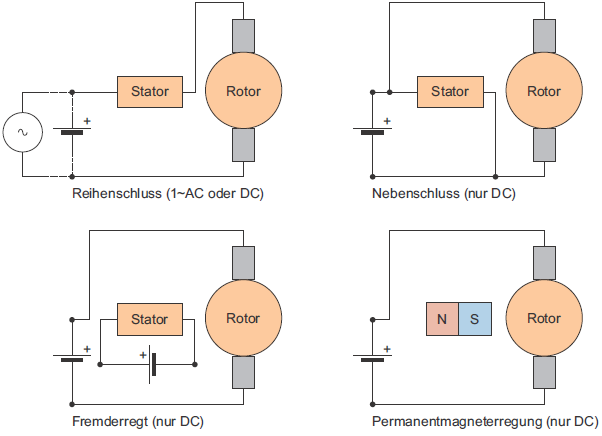
\includegraphics[width=150px]{Staenderaufbau.png}
			\subsection{Ersatzschaltbild}
				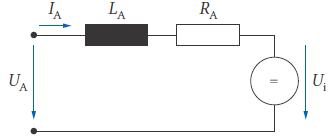
\includegraphics[width=120px]{DC_Ersatzschaltbild.png}
				\begin{symbolbox}
					\item Windungszahl im Anker: $w_A$
					\item $U_A = U_i +R_A\cdot I_A+L\cdot \frac{dI_A}{dt}$
					\item $U_i = c\cdot \phi \cdot \omega = c \cdot \phi \cdot 2\pi n = U_A - R_A\cdot I_A$
					\item $U_A = c\cdot \phi \cdot \omega +R_A\cdot I_A$
					\item $n_0 = \frac{U_i}{2\pi\cdot c\cdot \phi}$
					\item $R_A = \frac{P_{el}-P_n}{I_A^2} = \frac{-c\cdot \phi\cdot (2\cdot c\cdot \phi \cdot I\cdot \pi - U_A)}{M}$
					\item Proportionalitätskonstante: $c =\frac{4}{2\pi}\cdot w_A\cdot p$
					\item Inneres Drehmoment: $M_i = \frac{c\cdot \phi}{2\pi} \cdot I_A$
					\item $ P_{i, el} = P_{i, mech} = M_i \cdot \omega = U_i\cdot I_A$
					\item Haltedrehmoment: $M_H = c\cdot \phi \cdot \frac{U_A}{R}$
					\item $n(M_i) = \frac{U_A}{2\pi\cdot c\cdot \phi}-\frac{R_A}{2\pi(c\cdot \phi)^2}\cdot M_i$
					\item $M_i(n) = c\cdot \phi\cdot \frac{U_A}{R_A}-n\cdot \frac{2\pi(c\cdot \phi)^2}{R_A}$
					\item Anlaufdrehmoment: $M_i = \frac{c\cdot \phi \cdot U_A}{2\pi \cdot R_A}$
				\end{symbolbox}

				\begin{bluebox}{Nebenschluss-Motor}
					\item $c_n = c\cdot \frac{2\pi}{60\,s/min}$
					\item $M = c\cdot \phi \cdot I_A$
					\item $U_{ind} = c_n \cdot \phi \cdot n$
					\item $U = R_A\cdot I_A + U_{ind}$
					\item $n_N = \underbrace{\frac{60\,s/min\cdot U}{2\pi\cdot c\cdot \phi}}_{n_0, ideal}-\underbrace{\frac{60\,s/min\cdot M\cdot R_A}{2\pi\cdot(c\phi)^2}}_{\Delta_n}$
					\item $M = c_n\cdot \frac{60\,s/min}{2\pi}\cdot \frac{\phi}{R_A}\cdot (U-c_n\cdot \phi \cdot n)$
				\end{bluebox}

				\begin{symbolbox}{Reihenschluss-Motor}
					\item $c_n = c\cdot \frac{2\pi}{60\,s/min}$
					\item $c_{nR} = c_n \cdot k_r$ aus $\phi= k_r \cdot I$
					\item $M = c_{nR}\cdot \frac{2\pi}{60\,s/min}\cdot I^2$
					\item $U_{ind} = c_{Rn}\cdot I \cdot n$
					\item $n = \frac{U-I\cdot R_A}{c_{Rn}\cdot I}$
					\item $n = \frac{U}{\sqrt{c_{nR}\cdot \frac{60\,s/min}{2\pi} \cdot \sqrt{M}}}-\frac{R_A}{c_{nR}}$
				\end{symbolbox}
		\end{sectionbox}
	
% ======================================================================
% End
% ======================================================================
\end{document}